\begin{figure}[t]
\begin{minipage}{0.25\columnwidth}
\resizebox{\columnwidth}{!}{
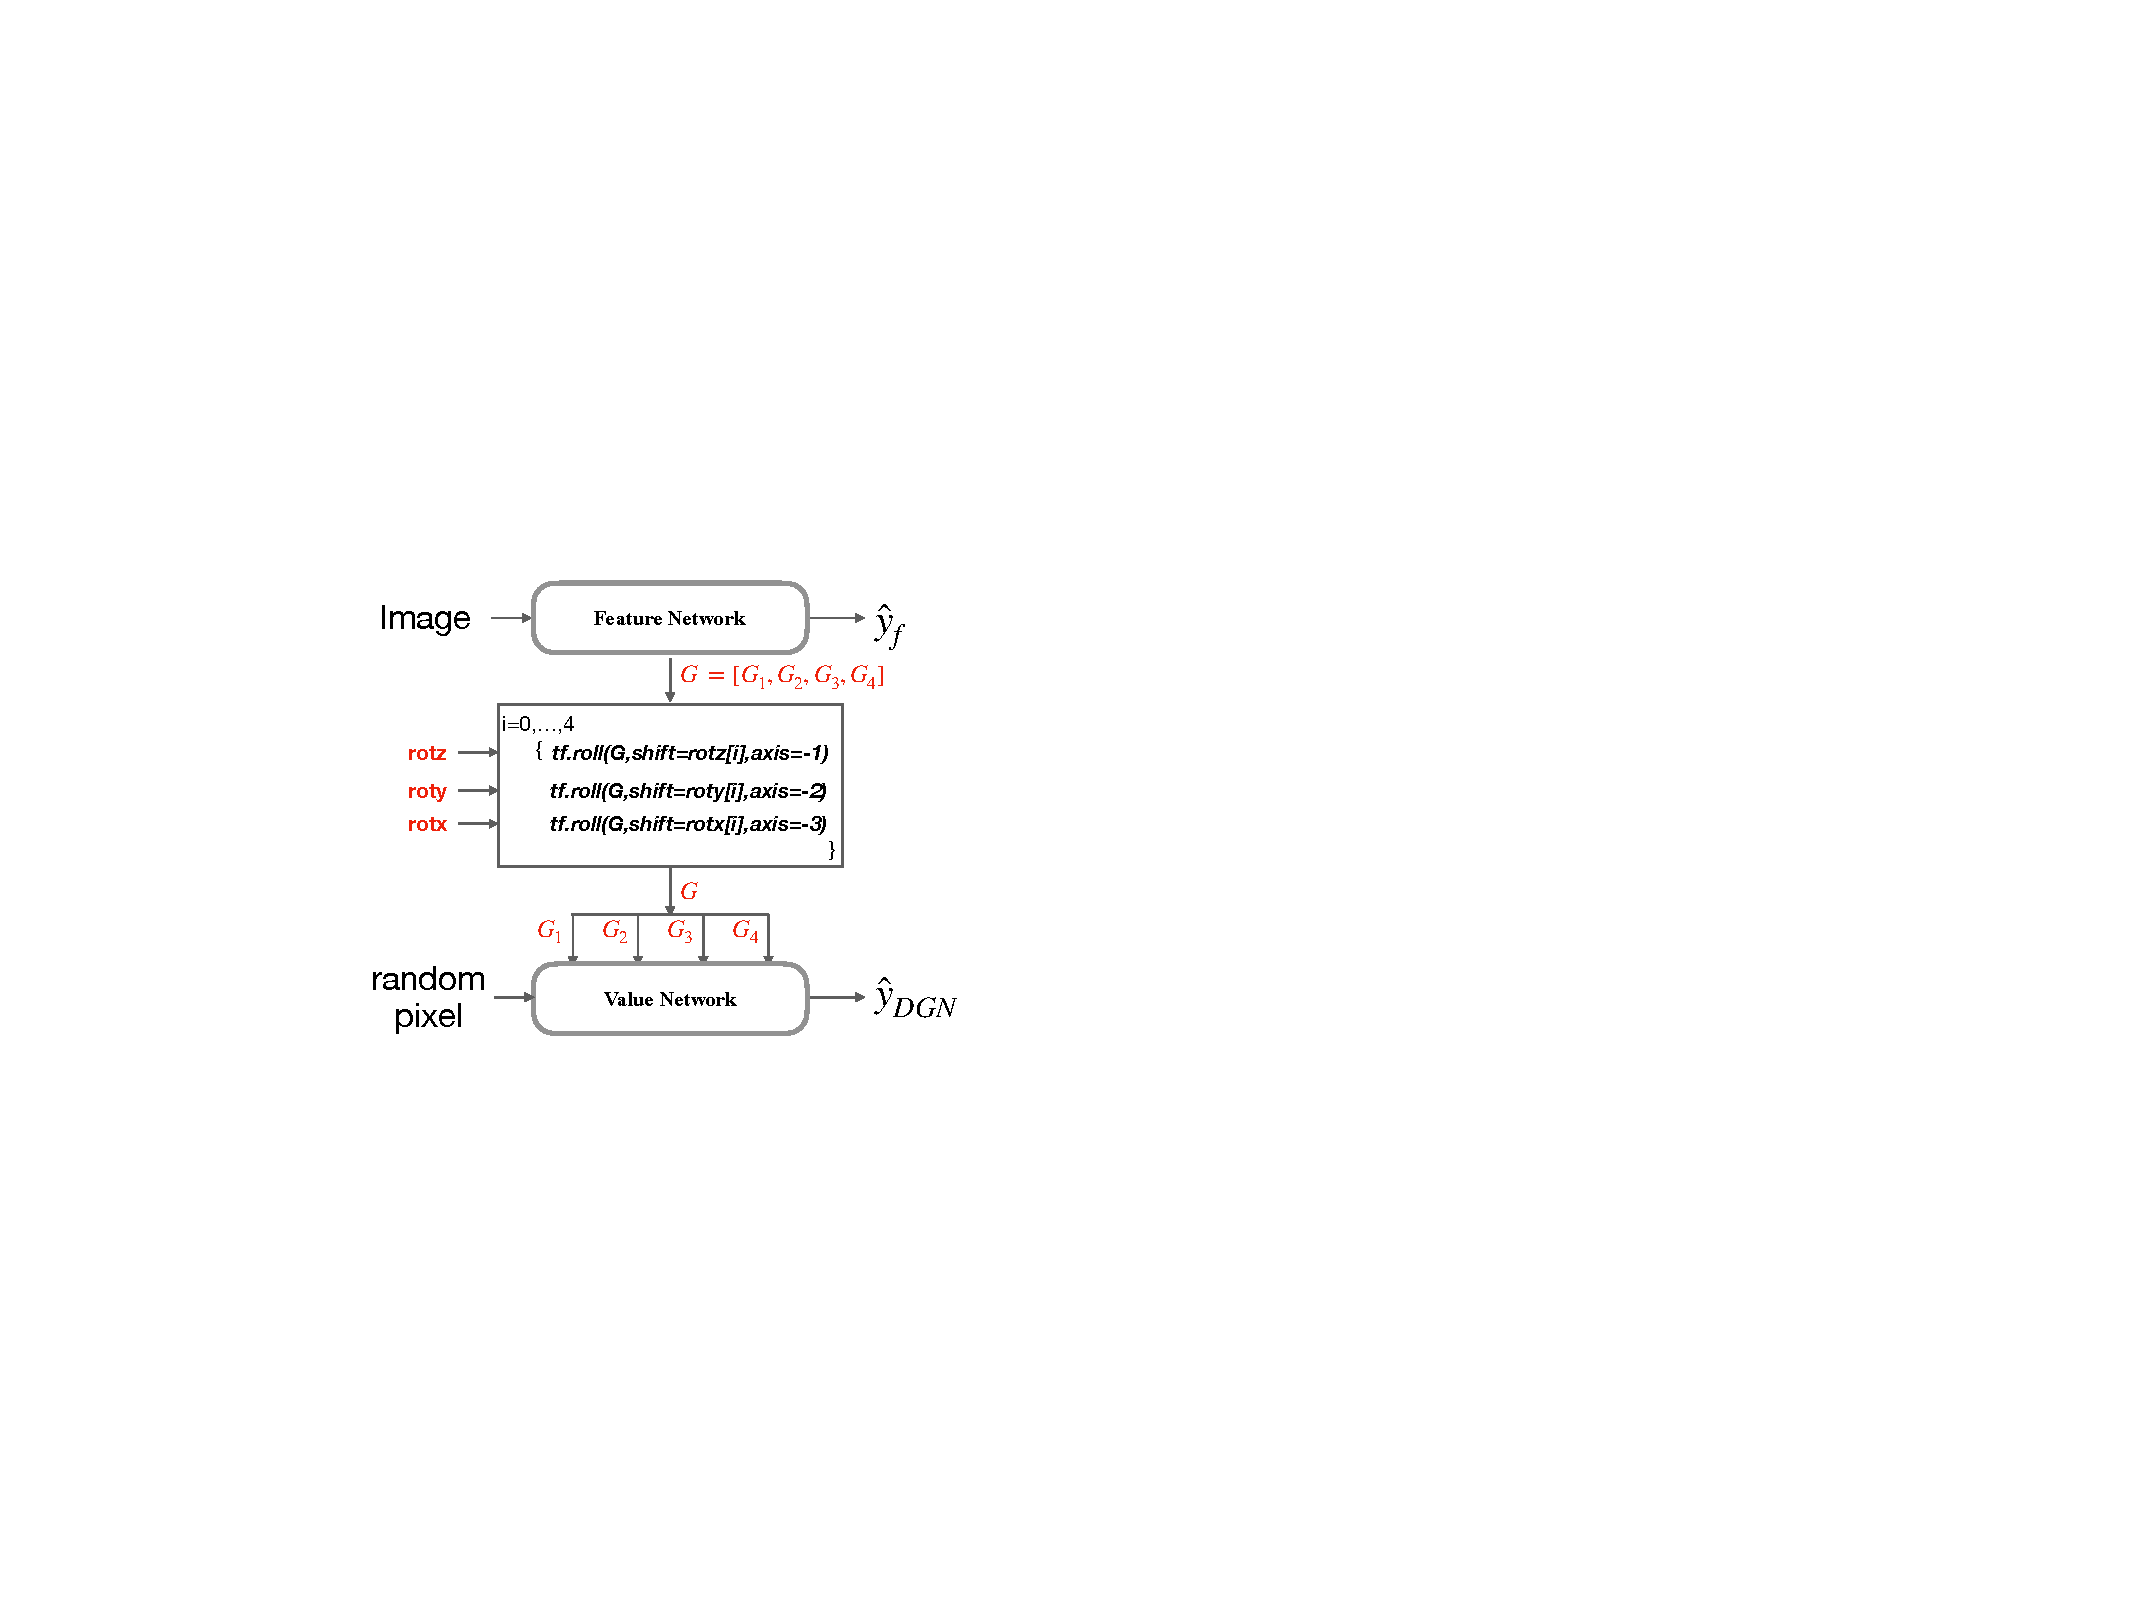
\includegraphics[scale=0.25]{figs/arbitrary_shift.pdf}
}
\end{minipage}
\begin{minipage}{0.68\columnwidth}
\resizebox{\columnwidth}{!}{
\begin{tabular}{c|c|cccccccc|c@{}}
&\resizebox{100pt}{!} {\Huge{Input}}& \resizebox{200pt}{!}{\Huge{Layer 1, Filter 1}}& \resizebox{200pt}{!}{\Huge{Layer 1, Filter 2}}&\resizebox{200pt}{!}{ \Huge{Layer 2, Filter 1}}& \resizebox{200pt}{!}{\Huge{Layer 2, Filter 2}}& \resizebox{200pt}{!}{\Huge{Layer 3, Filter 1}}& \resizebox{200pt}{!}{\Huge{Layer 3, Filter 2}}&\resizebox{200pt}{!}{\Huge{Layer 4, Filter 1}}& \resizebox{200pt}{!}{\Huge{Layer 4, Filter 2}}&\resizebox{180pt}{!}{\Huge{Test Acc.}}\\
\toprule
\resizebox{200pt}{!} {\shortstack{\Huge{Feature}\\\Huge Network\\\mbox{}\\\mbox{}\\\mbox{}\\\mbox{}\\\mbox{}\\\mbox{}\\\mbox{}}}&\includegraphics{visual-iclr/images/horse.png}&
\includegraphics{images_neurips_2021/feature_network/layer_1_0.png}&
\includegraphics{images_neurips_2021/feature_network/layer_1_1.png}&
\includegraphics{images_neurips_2021/feature_network/layer_2_0.png}&
\includegraphics{images_neurips_2021/feature_network/layer_2_1.png}&
\includegraphics{images_neurips_2021/feature_network/layer_3_0.png}&
\includegraphics{images_neurips_2021/feature_network/layer_3_1.png}&
\includegraphics{images_neurips_2021/feature_network/layer_4_0.png}&
\includegraphics{images_neurips_2021/feature_network/layer_4_1.png}&
{\resizebox{200pt}{!}{\shortstack{80.4\tiny$\pm$0.3\\\mbox{}\\\mbox{}\\\mbox{}\\\mbox{}}} }\\\hline
\resizebox{200pt}{!} {\shortstack{\Huge{Value}\\\Huge Network\\\mbox{}\\\mbox{}\\\mbox{}\\\mbox{}\\\mbox{}\\\mbox{}\\\mbox{}}}&\includegraphics{images_neurips_2021/allones.png}&
\includegraphics{images_neurips_2021/value_network//layer_1_0.png}&
\includegraphics{images_neurips_2021/value_network//layer_1_1.png}&
\includegraphics{images_neurips_2021/value_network//layer_2_0.png}&
\includegraphics{images_neurips_2021/value_network//layer_2_1.png}&
\includegraphics{images_neurips_2021/value_network//layer_3_0.png}&
\includegraphics{images_neurips_2021/value_network//layer_3_1.png}&
\includegraphics{images_neurips_2021/value_network//layer_4_0.png}&
\includegraphics{images_neurips_2021/value_network//layer_4_1.png}&
{\resizebox{200pt}{!}{\shortstack{79.4 \tiny$\pm$0.2\\\mbox{}\\\mbox{}\\\mbox{}\\\mbox{}}} }\\
\end{tabular}
}

\end{minipage}
\caption{\small On the left is the setup for arbitrary rotation of gates. On the right, we have the images related to feature and value networks on top and bottom rows respectively. Each row has the input image followed by the output of first $2$ filters in each of the $4$ layers.  In the bottom row, the input column `appears' blank because it is the image of the $\mathbf{1}$ input to the value network.  Despite the arbitrary rotation and $\mathbf{1}$ input,  the value network is within $1\%$ of  feature network's test accuracy (on CIFAR-10).}
\label{fig:visual-permute}
\end{figure}
